\documentclass[11pt,a4paper,english]{article}
\usepackage{geometry}
\geometry{a4paper}

\usepackage{color}
\usepackage{graphicx}
\usepackage{indentfirst}
\usepackage{amsmath}
\usepackage{multirow}
\usepackage{enumerate}
\usepackage{siunitx}
\usepackage[font=small,labelfont=bf,tableposition=top]{caption}
\usepackage{booktabs}
\usepackage[colorlinks,linkcolor=black]{hyperref}
\usepackage{threeparttable}
\newcommand{\tabincell}[2]{\begin{tabular}{@{}#1@{}}#2\end{tabular}}
\linespread{1.2}

\begin{document}

\vspace*{0.25cm}

\hrulefill

\thispagestyle{empty}

\begin{center}
\begin{large}
\sc{UM--SJTU Joint Institute \vspace{0.3em} \\ Probabilistic Methods in Engineering \\(Ve401)}
\end{large}

\hrulefill

\vspace*{5cm}
\begin{Large}
\sc{{Project Report}}
\end{Large}

\vspace{2em}

\begin{large}
\sc{{Term Project 2
\vspace{0.5em}

Police Shootings in the United States}} \\
\vspace{2em}
\end{large}
\today
\end{center}

\vfill

\begin{table}[h!]
\centering
\begin{tabular}{ll}
\textbf{Name} & \textbf{ID} \\
\textsc{Li Minhao} & \texttt{516370910223} \\
\textsc{Xie Mufeng} &  \texttt{515370910186} \\
\textsc{Yao Shaoxiong} & \texttt{517370910014} \\
\textsc{Zhang Zhenyuan} & \texttt{517370910124} \\
\textsc{Zhao Yijia} &  \texttt{517370910243} \\
\end{tabular}
\end{table}
\newpage
\begin{abstract}
\end{abstract}
\newpage
\tableofcontents
\newpage\section{Introduction}
Fatal police shootings are the incidents that police shoot the suspect to death in the line of duty. Constitutionally, police are allowed to shoot "to protect their life or the life of another innocent party" or "prevent a suspect from escaping if the suspect is thought to pose a threat to others"[2]. Their decisions are made under very tense circumstance and the justification is often controversial. The Washington Post started collecting the data of these incidents in 2015 and tried to appeal people to pay close attention to this issue. The Post obtained the data from four sources[3]: 
\begin{enumerate}[(i)]
    \item Local news reports
    \item Enforcement websites
    \item Social media
	\item Independent databases such as Killed by Police and Fatal Encounters
\end{enumerate}
The Post only documented those shootings in which ``a police officer, in the line of duty, shoots and kills a civilian"[3]. The incidents that were ``deaths of people in police custody, fatal shootings by off-duty officer or non-shooting deaths" were not included[3]. The data recorded by the Post started form 2015 and is still updating right now. From the source of the data, we can conclude that the incidents recorded by the Post were really severe. These incidents that threatened people's life possibly happened randomly. We can assume these incidents have following properties:
\begin{enumerate}
    \item Each incident did not influence other incidents and they were independently to happen.
    \item During a short period, the probability for one incident to occur is proportional to the length of time period. 
\end{enumerate}
Based on these assumption, we want to develop a comprehensive statistic model to predict the numbers of incidents happen in following time duration. We want to provide statistical analysis to indicate whether the shootings become more frequent or not. Our analysis can provide people with a better understanding of the fatal police shootings.
\section{Model Description}
From the assumptions we made in previous section, we use Poisson distribution to explain the occurrence of fatal police shootings in a given time duration. 
We will call the fatal police shootings by incident for short. 
The number of incidents is denoted as $X$. We assume $\lambda$ is the average number of incidents per day and $t$ is the number of days we observe, then the probability to have $n$ incidents happen will be 
\[P[X = n] = e^{-\lambda t}\frac{(\lambda t)^{n}}{n!}.\]
The expectation and variance of $X$ will be 
\[
    \begin{aligned}
        \text{E}[X] &= \lambda t,\\
        \text{Var}[X]&= \lambda t.\\
    \end{aligned}
\]

The data we got from the Post started from 2015 and ended in 2019 April. We will split them into two parts for estimation and prediction.

Our first step is to provide an estimation for parameter $\lambda$ based on the the data from 2015 to 2018. 
Then we perform a goodness-of-fit test to check whether our model is appropriate. 
We also take the influence of other factors like weekday into account. 
In this end, we carefully analyze the confidence interval for $\lambda$ and the prediction interval of $X$ in 2019. 
We compare our results with real observations and make an evaluation to our model. 
\subsection{Notations}
To make our discussion clear, we summarize notations we will use in the following table.
\begin{table}[htbp]
	\centering
	\caption{Notations in this report.}
	\begin{tabular}{cc}
		\hline
		Notation & Meaning of the notation\\
		\hline
		$t$ & Number of observation days.\\
		$n$ & Number of incidents happened in observation.\\
		$X$ & Random variable for the number of incidents.\\
		$X_{ob}$ & Observed number of incidents during observation.\\
		$\bar{X}$ & Random variable for the number of incidents per day during observation.\\
		$\bar{X}_{ob}$ & Observed number of numbers incidents per day during observation.\\
		$\lambda$ & Parameter of Poisson distribution in the model, unit is $\text{day}^{-1}$.\\
		$\hat{\lambda}$ & Estimated value of $\lambda$.\\
		$k$ & Parameter of Poisson distribution in the model, $k = \lambda t$.\\
		$\hat{k}$ & Estimated value of $k$.\\
		$\chi_{\nu}^{2}$ & Chi-squared distribution with $\nu$ degrees of freedom.\\
		\hline
	\end{tabular}
\end{table}
\section{Estimation for Parameter in the Model}
To summarize the data we got from the Washington Post, we plot a figure to show the number of incidents happened in a day with respect to the date. The data we covered here are from 2015 to 2018.
\begin{figure}[htbp]
	\centering
	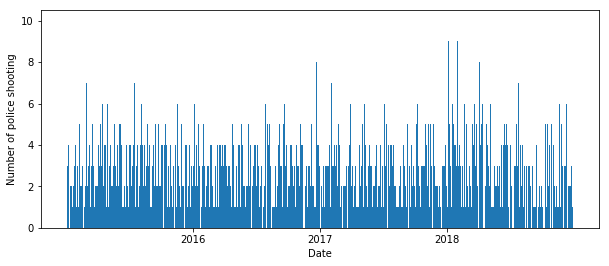
\includegraphics[width = \textwidth]{1.png}
    \caption{Number of incidents happened per day with respect to the date from 2015 to 2018.}
\end{figure}

From a general observation, the distirbution of incidents is approximately uniform. This motivates us to estimate parameter $\lambda$ in our model.

We know that $E[X] = \lambda t$, so for a fixed time period, 
\[\hat{\lambda} = \frac{X}{t}\]
will be an unbiased estimator for $\lambda$.

The unit of $\hat{\lambda}$ is $\text{day}^{-1}$ here and this will make the value neither too large nor too small. For this period of observation, we have 
\begin{align*}
	t &= 1461\text{ days},\\
	X_{ob} &= 3943.
\end{align*}
Then the estimated value of $\lambda$ is
\[\hat{\lambda} = \frac{X_{ob}}{t} \approx 2.70.\] 

\section{Goodness-of-Fit Test}
After we fit the parameter in our model, we want to further test whether our model is actually appropriate. We use a goodness-of-fit test here and the null hypothesis is
\[H_{0}:\text{Poisson distribution is an appropriate model.}\]

To make further quantitative discussion, we need to divide these days into different categories. 
From the assumption of our model, the number of incidents happened in a day will also follow a Poisson distribution with $t = 1\text{ day}$. 
And the observation in each day is independent and identical. We use the number of incidents in a day to categorize these days.

Since there is no day that has more than 10 incidents, we decide to make 11 categories. Now we need to calculate the probability for one day to fall into each category. Using Poisson distribution, we take number of incidents equal to $2$ as an example
\[
	\begin{aligned}
		P[X = 2] &= \frac{(\hat{\lambda}\times 1)^{2}}{2!}e^{-\hat{\lambda} \times 1}\\
		&= 0.245.\\
	\end{aligned}
\]

So the probability to have two incidents in a day from our model is $0.245$.
Based on similar calculation, the probability to have one day into each category is summarize in the following table:
\begin{table}[htbp]
    \centering
    \caption{Probability to have $n$ incidents happened in a day predicted from our model.}
	\begin{tabular}{c|cccccc}
		\hline
		\# of incidents, $n$ & 0 & 1 & 2 & 3 & 4 & 5\\
		\hline
		$P[X = n]$ & 0.067 & 0.182 & 0.245 & 0.220 & 0.149 & 0.080\\ 
		\hline
		\# of incidents, $n$  & 6 & 7 & 8 & 9 & $\geq$10 & \\
		\hline
		$P[X = n]$  & 0.036 & 0.014 & 0.005 & 0.0014 & 0.0005 & \\ 
		\hline
    \end{tabular}
\end{table}

In this test, the quantity that will be directly used is the number of days expected in each category. We also summarize them in the following table.

\begin{table}[htbp]
    \centering
    \caption{Probability to have $n$ incidents happened in a day predicted from our model.}
	\begin{tabular}{c|cccccc}
		\hline
		\# of incidents, $n$ & 0 & 1 & 2 & 3 & 4 & 5\\
		\hline
		$E_{i}$ & 98.2 & 265.1 & 357.9 & 322.1 & 217.4 & 117.4\\ 
		\hline
		\# of incidents, $n$  & 6 & 7 & 8 & 9 & $\geq$10 & \\
		\hline
		$E_{i}$  & 52.8 & 20.4 & 6.9 & 2.1 & 0.73 & \\ 
		\hline
    \end{tabular}
\end{table}

We can notice that for all the categories such that $E_{i} \geq 5$ are 9 out of 11. This satisfies the requirement $E_{i} \geq 5$ for 80\% categories.

The Pearson statistic will approximately follow a chi-squared distribution in this case. Since we have 11 categories in total, the chi-squared random variable has $11-1-1 = 9$ degree of freedom[4].
\[X^{2}_{9} = \sum_{i = 0}^{9}
\frac{(O_{i}-E_{i})^{2}}{E_{i}} \sim \chi_{9}^{2}\]

For out test, we choose the significance level $\alpha = 0.05$. If $X^{2}_{9} > \chi_{0.05,9}^{2}$, we will reject $H_{0}$ ; otherwise we will accept $H_{0}$.

Since the data we obtain consist of four years from 2015 to 2018, we would like to do the test for four years together first and test one year to confirm our result. 
\subsection{Test for Observations in Four Years Together}
We summarize the numbers of days in each category observed and estimated from 2015 to 2018 in the following table.
\begin{table}[htbp]
    \centering
    \caption{Number of days in each category observed and esitmated from 2015 to 2018.}
	\begin{tabular}{c|cccccc}
		\hline
        \# of incidents, $n$ & 0 & 1 & 2 & 3 & 4 & 5 \\
		\hline
		$O_{i}$ & 108 & 287 & 324 & 310 & 227 & 116\\
		\hline
		$E_{i}$ & 98.2 & 265.1 & 357.9 & 322.1 & 217.4 & 117.4\\ 
		\hline
		\hline
		\# of incidents, $n$ & 6 & 7 & 8 & 9 & $\geq 10$ & \\
		\hline
		$O_{i}$ & 53 & 21 & 11 & 3 & 1 &\\
		\hline
		$E_{i}$  & 52.8 & 20.4 & 6.9 & 2.1 & 0.73 & \\ 
		\hline 
    \end{tabular}
\end{table}

We then calculate the Pearson statistic,
\[
	\begin{aligned}
		X_{9}^{2} &= \sum_{i = 0}^{10}\frac{(O_{i}-E_{i})^{2}}{E_{i}}\\
		&= \frac{(108-98.2)^{2}}{98.2}+\cdots+\frac{(1-2.1)^{2}}{2.1}\\
		&\approx 9.91.\\
	\end{aligned}
\] 
However, we have $\chi^{2}_{0.05,10} = 16.92$, so since 
\[X_{9}^{2} = 9.91 < 16.92 = \chi_{0.05,9}^{2}\]
we accept $H_{0}$.

We also plot number of days in each category as a histogram for both the real case and predicted result. Observed case is shown in Figure 2 and predicted data is shown in Figure 3.
\begin{figure}[htbp]
	\centering
	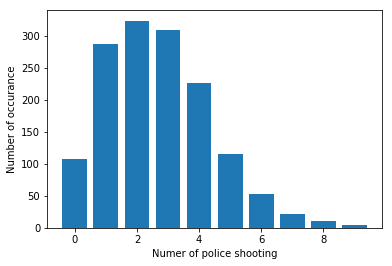
\includegraphics[width = \textwidth]{4-years.png}
	\caption{Number of days in each category in observation for 4 years together.}
\end{figure}
\begin{figure}[htbp]
	\centering
	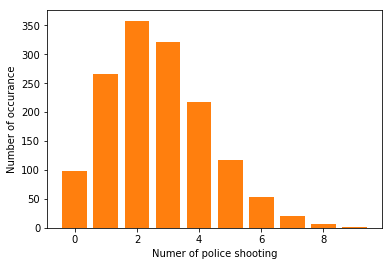
\includegraphics[width = \textwidth]{poisson.png}
	\caption{Number of days in each category from prediction for 4 years together.}
\end{figure}

From observation, we can notice that there is no significant difference between these two distributions. We confirm the result that Poisson distribution is an appropriate model.
\subsubsection{Test for Obervations in One Year}
Although we do not reject $H_{0}$ from the data from 4 years together, we want to test the hypothesis individually for one year to make sure our model is appropriate. We randomly pick year 2015 for test. We will first summarize $O_{i}$ and $E_{i}$ in a table and then do the hypothesis test.


\begin{table}[htbp]
    \centering
    \caption{Number of days in each category observed and esitmated in 2015-2018.}
	\begin{tabular}{c|cccccc}
		\hline
        \# of incidents, $n$ & 0 & 1 & 2 & 3 & 4  \\
		\hline
		$O_{i}$ & 24 & 73 & 87 & 69 & 55 \\
		\hline
		$E_{i}$ & 24.5 & 66.2 & 89.4 & 80.5 & 54.3 \\ 
		\hline
		\hline
		\# of incidents, $n$ & 5 & 6 & 7 & 8 & $\geq 9$  \\
		\hline
		$O_{i}$ & 33 & 14 & 8 & 2 & 0\\
		\hline
		$E_{i}$ & 29.3 & 13.2 & 5.1 & 1.7 & 0.70\\ 
		\hline 
    \end{tabular}
\end{table}

Here, since $E_{8}$, $E_{9}$ and $E_{10}$ do not satisfies $E_{i} \geq 5$, we merge $E_{9}$ and $E_{10}$ into one category. 
We apply the same method for all subsequent years. Then the degree of freedom for chi-squared random variable will be $10-1-1 = 8$.

We then calculate the Pearson statistic as follows,
\[
	\begin{aligned}
		X_{8}^{2} &= \sum_{i = 0}^{9}\frac{(O_{i}-E_{i})^{2}}{E_{i}}\\
		&= \frac{(24-24.5)^{2}}{24.5}+\cdots+\frac{(0-0.70)^{2}}{0.70}\\
		&\approx 6.14.\\
	\end{aligned}
\] 

For chi-squared distribution with degree 8, we have $\chi_{0.05,8}^{2} = 15.5$. So for the test of year 2015
\[X_{8}^{2} = 6.14 < \chi_{0.05,8}^{2} = 15.5,\]
so we cannot reject $H_{0}$ with significance 0.05.

In conclusion for this section, the hypothesis tests show that there is no significant evidence that the distribution of shooting incidents does not follow a Poisson distribution. We will use our model to do further calculation.
\section{Dependence on Other Factors}
In previous section, we confirm that our model is appropriate, but Poisson distribution assumes that the happening of police shooting is uniformly random. 

However, we think this may not be a complete description. 
The probability for an incident to happen may depend on weekday, but for the observation in a whole year, we approximately have number of different weekdays equal. 
So we wank to check the influence of other factors in this section and make the description of our model more appropriate. 
\subsection{Dependence on Weekdays}
We want to check whether the probability for an incident to happen depends on weekdays. We first plot the number of incidents happened in each weekday to have a general observation. The data we use here is the data for 4 years from 2015 to 2018 together.
\begin{figure}[htbp]
	\centering
	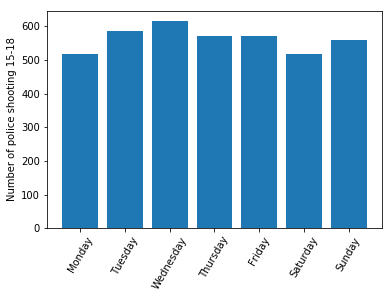
\includegraphics[width = 10cm]{weekdays.png}
	\caption{Number of incidents in each weekday for four years together.}
\end{figure}

From general observation, we cannot give a conclusion directly. So we will do a null hypothesis test to check the dependence. The null hypothesis test we formulated is 
\[H_{0}:\text{ The probability for an incident ot happen does not depend on weekday.}\]

We decide to choose significance level $\alpha = 0.05$ for our test.

If the null hypothesis is true, the probability for an incident to happen on each weekday will be equal, 
\[P_{1} = \cdots = P_{7} = \frac{1}{7}.\]

In these four years, there are 208  Tuesdays and Wednesdays; there are 209 other weekdays. 
Since the difference is relative small, we ignore the difference of the numbers of weekdays.
So if the null hypothesis holds, we will have expected number of incidents happened in each weekday equal to 
\[E_{i} = P_{i} \times N = \frac{N}{7}.\]

In the following table, we list the number of incidents happened in each weekday by observation and by prediction. 
Here we use the fact the total number of incidents is $N = 3943$.
\begin{table}[htbp]
	\centering
	\caption{Number of incidents happened in each weekday by observation and by prediction.}
	\begin{tabular}{c|ccccccc}
		\hline
		Weekday & Mon. & Tue. & Wed. & Thur. & Fri. & Sat. & Sun.\\
		\hline
		$O_{i}$ & 517 & 586 & 616 & 573 & 572 & 518 & 561\\
		\hline
		$E_{i}$ & 563.29 & 563.29 & 563.29 & 563.29 & 563.29 & 563.29 & 563.29\\
		\hline
	\end{tabular}
\end{table}

We can notice that for each category $E_{i} > 5$, so the Pearson statistic 
\[X^{2}_{6} = \sum_{i = 1}^{7}\frac{(O_{i}-E_{i})^{2}}{E_{i}} \sim \chi^{2}_{6}\]
will approximately follow a chi-squared distribution with $7-1 = 6$ degrees of freedom. 
To reject the null hypothesis with significance level $\alpha = 0.05$, we need the Pearson statistic satisfies
\[X^{2}_{6} > \chi^{2}_{0.05,6} = 12.592.\]

From calculation, 
\[
	\begin{aligned}
		X^{2}_{6} &= \frac{(517-563.29)^{2}}{563.29}+\cdots+\frac{(561-563.29)^{2}}{563.29}\\
		&\approx 13.605.\\
	\end{aligned}
\]

So we have $X^{2}_{6} > \chi^{2}_{0.05,6}$ and we can reject $H_{0}$.

From our test, we can conclude that there is evidence that the probability for an incident to happen is not independent to weekday. In other word, the probability for an incident to happen will probably depend on weekday.

\subsection{Probability for Incidents to happen on Wednesdays and Mondays}
To make our conclusion more appropriate, we want to check the probability for an incident to happen on two weekdays. 
We choose Wednesday and Monday to do the test because they have maximum and minimum numbers of incidents happened.

Here we choose to summarize the number of incidents happened per day for Wednesday and Monday. We also plot the distribution in the following diagram.
\iffalse
\begin{table}[htbp]
	\centering
	\caption{Number of incidents happened per day for Wednesday and Monday.}
	\begin{tabular}
	\end{tabular}
\end{table}
\begin{figure}[htbp]
	\centering
	\caption{Number of incidents happened per day for Wednesday.}
\end{figure}
\begin{figure}[htbp]
	\centering
	\caption{Number of incidents happened per day for Wednesday.}
\end{figure}
\fi

From general observation, the distributions of incidents per day seem to be the same. However, we need to do a hypothesis test to make an appropriate conclusion.

Here we omit the part to check these two distributions are both Poisson distribution with significance level $\alpha = 0.05$. From our test, there are no evident that these two distributions are not Poisson distributions.

Our focus will be whether these two distributions are different. The null hypothesis we have is 
\[H_{0}:\text{ These two distributions are the same Poisson distribution.}\]
The significance level we choose here is $\alpha = 0.05$.

If this null hypothesis is true, they will have the same parameter, i.e.,
\[\lambda_{1} = \lambda_{2}.\]
Then for the estimators we use, they will have the relation 
\[E[\hat{\lambda_{1}}-\hat{\lambda_{2}}] = 0,\]
since $\hat{\lambda_{1}}$ and $\hat{\lambda_{2}}$ are unbiased estimators for $\lambda_{1}$ and $\lambda_{2}$.

The samples we use in this test is large enough, then from Central Limit theorem[4] we have 
\[\frac{\hat{\lambda_{1}}-\hat{\lambda_{2}}}{\sqrt{\text{Var }(\hat{\lambda_{1}-\hat{\lambda_{2}}})}}\sim N(0,1),\]
here $N(0,1)$ is s standard normal distribution.

The variance of variable $\hat{\lambda_{1}}-\hat{\lambda_{2}}$ is estimated from observation, an unbiased estimator is derived from
\[
	\begin{aligned}
		\text{Var }((\hat{\lambda_{1}}-\hat{\lambda_{2}}) &= \text{Var }(\frac{X_{1}}{t_{1}}-\frac{X_{2}}{t_{2}})\\
		&= \frac{1}{t_{1}^{2}}\times \text{Var }X_{1}+\frac{1}{t_{2}^{2}}\times \text{Var }X_{2}\\
		&= \lambda_{1} t_{1}+\lambda_{2} t_{2}.
	\end{aligned}
\]
Here we use the fact that $X_{1}$ and $X_{2}$ are independent. So we use $\hat{\lambda_{1}}t_{1}+\hat{\lambda_{2}}t_{2}$ to estimate $\text{Var }(\hat{\lambda_{1}}-\hat{\lambda_{2}})$.
\section{Confidence Interval for $k$}

\section{Prediction Interval}
We denote the number of observations in following time $t$ as $Y$.
To predict the number of observations in the following time period, we need to find the distribution of $\hat{Y}$ related to $Y$. 
From Poisson distribution, we know the expectation and variance for $Y$ with observation time $t$ are
\begin{align*}
	\text{E}[Y] &= \lambda t,\\
	\text{Var}[Y] &= \lambda t.\\
\end{align*}
The estimator we chose for $\lambda$ is based the number of observations happened before we observe $Y$.
We denote the length of observation $s$ and number of observations $X$, then
\begin{equation*}
	\hat{\lambda} = \frac{X}{s}.
\end{equation*}
We choose the estimator for $Y$ denoted $\hat{Y}$ to be $\hat{\lambda}t$.
Note that
\begin{align*}
	\text{E}[Y-\hat{\lambda}t] &= \text{E}[Y]-\text{E}[X]\frac{t}{s}\\
	&= \lambda t-\lambda s \cdot \frac{t}{s}\\
	&= 0.
\end{align*}
If $\lambda t$ and $\lambda s$ are both large enough, the random variable $Y$ and $\hat{\lambda}t$ will both follow a normal distribution and their difference is also a normal distribution.
The mean of $Y-\hat{\lambda}t$ is $0$, and for the variance
\begin{align*}
	\text{Var}[Y-\hat{\lambda}t] &= \text{Var}[Y]-\text{Var}[\hat{\lambda}t]\\
	&= \lambda t+\frac{t^{2}}{s}\lambda.\\
\end{align*}
Here we use the fact that $X$ and $Y$ for different periods of observations are independent.
This gives the derivation of Nelson's formula [1,(18)].
Then we use estimated $\hat{\lambda}$ to replace $\lambda$ and 
\begin{equation*}
	\frac{Y-\hat{\lambda}t}{\sqrt{\hat{\lambda}\left(t+\frac{t^{2}}{s}\right)}} \sim N(0,1).
\end{equation*}
The prediction interval of $Y$ with \SI{95}{\percent} confidence will be 
\begin{equation*}
	\left[
	\hat{\lambda}t-z_{0.025}\sqrt{\hat{\lambda}\left(t+\frac{t^{2}}{s}\right)},
	\,
	\hat{\lambda}t+z_{0.025}\sqrt{\hat{\lambda}\left(t+\frac{t^{2}}{s}\right)}
	\right].
\end{equation*}
We then plug in the number of observations happened in 2015-2018 and get the estimated $\hat{\lambda}$ first,
\[\hat{\lambda} = .\]

\section{Discussion}
\section{Summary}
\section{Reference}
[2] Police can use deadly force if they merely perceive a threat. \href{https://www.vox.com/identities/2016/8/13/17938226/police-shootings-killings-law-legal-standard-garner-graham-connor}{https://www.vox.com/identities/2016/8/13/17938226}

[3] How The Washington Post is examining police shootings in the United States. \href{https://www.washingtonpost .com/national/how-the-washington-post-is-examining-police-shootings-in-the-united-states/2016/07/07/d9c52238-43ad-11e6-8856-f26de2537a9d_story.html?utm_term=.bb540299ce96}{https://www.washingtonpost .com/national}
\end{document}
